\chapter{Literatuurstudie}
\label{ch:stand-van-zaken}

% Tip: Begin elk hoofdstuk met een paragraaf inleiding die beschrijft hoe
% dit hoofdstuk past binnen het geheel van de bachelorproef. Geef in het
% bijzonder aan wat de link is met het vorige en volgende hoofdstuk.

% Pas na deze inleidende paragraaf komt de eerste sectiehoofding.
\paragraph{Inleiding}
Zoals eerder vermeld wordt er gebruik gemaakt van twee React-Redux projecten. In dit hoofdstuk wordt meer informatie gegeven omtrent de achtergrond van deze projecten en wat er nodig is om deze met elkaar te laten communiceren. React bestaat uit JavaScript en om een hogere compatibiliteit te verkrijgen wordt JSX gebruikt omdat deze HTML syntax kan laten bestaan met JavaScript code. Conceptueel bestaat React uit components, elk deel functionaliteit zal een component zijn. Dit voorhoogt ook de herbruikbaarheid van de code. Deze components hebben een lifecycle die doorlopen wordt met een initialisatie, een mount fase, een update en een unmount fase. Daarnaast wordt gebruik gemaakt van Redux om makkelijk de state van de applicatie te beheren. In grote projecten kan het soms moeilijk zijn om te weten wat er waar precies aan het gebeuren is. Om deze state te beheren wordt er hier ook gebruik gemaakt van een bepaalde flow. Container components gaan meestal zorgen voor de connectie tussen React en Redux. 

\section{React}
Volgens \autocite{React01} is React een JavaScript library om user interfaces te bouwen. React is component-based. Een component implementeert een \textit{render} methode die data als input neemt en een view retourneert. Om dit te doen wordt JSX gebruikt. Er kunnen simpele views gemaakt worden voor elke state van de applicatie en React zal deze updaten en de juiste componenten renderen wanneer de data verandert.

\subsection{JSX}
JSX is een XML/HTML-achtige syntax gebruikt door React die ECMAScript uitbreidt zodat XML/HTML-achtige text kan bestaan met JavaScript/React code. Deze syntax is bedoeld om gebruikt te worden door preprocessoren (zoals Babel) om HTML text gevonden in JavaScript files om te zetten in standaard JavaScript objecten. Dit wil dus zeggen dat je door JSX te gebruiken HTML structuren en JavaScript code kan schrijven in dezelfde file, Babel zal dan alle uitdrukkingen vertalen naar JavaScript code. Waar vroeger dus JavaScript code in HTML werd geplaatst, laat JSX het toe om HTML in JavaScript te plaatsen.
\autocite{jsx}

\subsection{Components}
Een enkele view van een user interface is opgedeeld in een aantal stukken, in een aantal components. De start component bevat een tree, die tree kan opgedeeld worden in een aantal sub-components. Deze kunnen dan weer opgedeeld worden in nog meer sub-components. Dit kan dus resulteren in een complexe tree met verschillende React components. Er zijn echter ook nog verschillende soorten components, namelijk \textit{simple} en \textit{stateful}. 
\autocite{jsx}

\paragraph{Simple component}
React components implementeren de \textit{render} methode, ze retourneren wat er moet afgebeeld worden. Daarvoor wordt het eerder aangekaarte JSX gebruikt. Input data die doorgegeven is aan de component kan worden opgeroepen door de \textit{props} aan te spreken van deze component. Sidenote: JSX is optioneel, het gewenste resultaat kan ook bereikt worden door JavaScript code alleen. JSX maakt het wel overzichtelijker om de props aan te spreken.  
\autocite{React01}

\paragraph{Stateful component}
In toevoeging met data als input nemen (via \textit{props}), kan een component zijn interne state aanspreken om daar data uit te halen. Wanneer de data uit de state van een component verandert, wordt de render methode opnieuw aangeroepen zodat de juiste data getoond wordt.
\autocite{React01}




\subsection{React lifecycle}
Met React is het mogelijk om components te creëren door de voorziene methode van React te gebruiken. Deze methode verwacht een \textit{render} methode en zal een lifecycle triggeren, de lifecycle van een component. 
Deze lifecycle kan onderverdeeld worden in 4 grote fasen zoals beschreven in figuur 1.1 en 1.2:
\newline
\begin{itemize}
	\item initialisatie
	\item mounten
	\item updaten
	\item unmounten
\end{itemize}
\begin{figure}
	\begin{center}
		\caption{De initialisatie en de mounting fase van de React lifecycle. Verkregen van \textcite{reactlifecycle}.}
		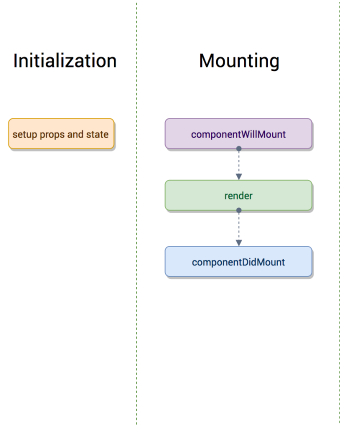
\includegraphics[width=8cm]{img/react-lifecycle1}\\[0.5cm]
	\end{center}
\end{figure}

\begin{figure}
	\begin{center}
		\caption{De update en de unmount fase van de React lifecycle. Verkregen van \textcite{reactlifecycle}.}
		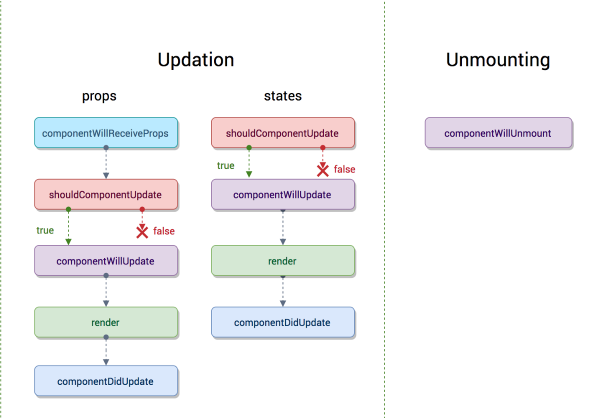
\includegraphics[width=15cm]{img/react-lifecycle2}\\[0.5cm]
	\end{center}
\end{figure}

\paragraph{Initialisatie}
In deze fase worden de initiële state en de default props ingesteld. De initiële state wordt in de constructor ingesteld, deze kan later altijd veranderd worden door de \textit{setState} methode. \textit{defaultProps} is een property van \textit{Component} die overschreven kan worden met nieuwe waarden voor de props. 

\paragraph{Mounten}
In de tweede fase zijn er een aantal \textit{hook} methodes die aangeroepen kunnen worden voor het mounten en na het mounten. Een hook methode is een methode waar je kan inpikken in de lifecycle en bestaande code kan veranderen of verbeteren naar eigen noden. 

Al de dingen die moeten gebeuren voor een component gaat mounten, moeten gedefinieerd zijn in de \textit{componentWillMount}. Deze methode wordt een keer per lifecycle uitgevoerd voor de eerste \textit{render}. 

Render zal de component mounten in de browser. Het is een pure methode, dus het geeft altijd dezelfde output gegeven dezelfde input. 

Na deze eerste render, wordt de methode \textit{componentDidMount} aangeroepen. Deze methode wordt opnieuw een keer per lifecycle uitgevoerd. 

\paragraph{Updaten}
Deze derde fase start wanneer de React component succesvol gerenderd is op de browser. De component kan nu geüpdatet worden op twee manieren: het verzenden van nieuwe props of het updaten van de state. 

Wanneer de component nieuwe props ontvangt of de state is geüpdatet, wordt in de methode \textit{shouldComponentUpdate} gevraagd of er een re-render moet gebeuren of niet. Deze methode retourneert dus een boolean en zal standaard re-renderen tenzij anders beschreven. Het is dus mogelijk om enkel een re-render uit te voeren als de props veranderen. Deze hook methode wordt vooral gebruikt als renderen een zware methode is. Dan is het niet voordelig om altijd alles opnieuw te renderen.

Als de uitkomst van deze methode true is, dan zal de component updaten en wordt de hook methode \textit{componentWillUpdate} opgeroepen. In deze methode worden de nodige voorbereidingen gedaan voor de volgende render, gelijkaardig als \textit{componentWillMount}. Hierna wordt de component dus opnieuw gerenderd. 

Wanneer dit succesvol is dan zal \textit{componentDidUpdate} de third party libraries updaten en reloaden. 

Wanneer echter de props veranderen en het is niet de eerste render dan zal in \textit{componentWillReceiveProps} de state en de props opnieuw gesynchroniseerd worden met elkaar. 

\paragraph{Unmounten}
In de laatste fase is de component niet meer nodig en zal deze via \textit{componentWillUnmount} verwijderd worden. Hier kan er dan een cleanup gebeuren wat betreft user details en authorization tokens.
\autocite{reactlifecycle}
\autocite{reactlifecycle2}


\section{Redux}
De requirements voor JavaScript single-page applicaties worden meer en meer gecompliceerd. De code moet veel meer state beheren dan vroeger. Deze state kan server responses en gecachete data, maar ook lokaal gecreëerde data die nog niet naar de server is doorgestuurd bevatten. Deze steeds veranderende state beheren is moeilijk. Als een model een ander model kan updaten, waar een view dan een ander model kan updaten, die een nieuw model gaat updaten, die op zijn beurt ook nog eens een view kan updaten. Op een gegeven moment wordt het niet meer duidelijk wat er gebeurt in de applicatie. Wanneer een systeem ondoorzichtig en niet-deterministisch is, wordt het moeilijk om bugs te reproduceren of om nieuwe features toe te voegen. Deze complexiteit is moeilijk om mee om te gaan omdat er twee concepten in verwikkeld worden die moeilijk vatbaar zijn: mutatie en asynchroniteit. Beide kunnen apart heel handig zijn, maar samen kan dit voor heel wat problemen zorgen.

Door stateful components die elkaar aanroepen verhoogt de complexiteit om de state te beheren. Om tegen te gaan dat de controle verloren gaat over wanneer, hoe en waarom de state geüpdatet wordt, kan redux geïntroduceerd worden als oplossing om de state te managen. Redux zal proberen om de veranderingen op de state voorspelbaar te maken door bepaalde restricties op te leggen omtrent het updaten van de state. Deze restricties staan beschreven in de \textit{drie principes} van Redux.

\subsection{Drie principes}

\paragraph{Een enkele source}  
De state van de hele applicatie zit in een object tree in een enkele \textit{store}. Een enkele state maakt het makkelijker om te debuggen of om de applicatie te inspecteren. Sommige functionaliteit kan snel geïmplementeerd worden hierdoor, zoals een undo/redo waar dan geswitched kan worden tussen een vorige en een volgende state van de applicatie. Dit kan dus enkel wanneer de hele state van de applicatie is opgeslagen in de object tree.

\paragraph{State is read-only}
De enige manier om een state te veranderen is door het verzenden van een \textit{action}, dit is een object dat beschrijft wat er gebeurt. Dit zorgt ervoor dat callbacks nooit direct naar de state gaan schrijven. Ze tonen de intentie om de state te transformeren. Alle veranderingen zijn gecentraliseerd en gebeuren een voor een in een vaste volgorde.   

\paragraph{Pure functies voor veranderingen}
Om te specificeren hoe de state tree veranderd is ten gevolge van actions, worden pure \textit{reducers} geschreven. Reducers zijn pure functies die dan geëxporteerd worden. Ze nemen de vorige state en de action om zo de volgende state te retourneren. Het is belangrijk om een nieuw state object te retourneren in plaats van het muteren van de vorige state. 

\subparagraph{Pure functie}
Een pure functie is een functie die met dezelfde input altijd dezelfde output produceert.
\autocite{Pure01}

Redux draait nu net om de voorspelbaarheid en betrouwbaarheid. Door een mutatie kan deze state niet meer voorspelbaar of betrouwbaar zijn. 

\subsection{Redux flow}
In de subsectie \textit{Drie principes} kwamen een aantal core concepts voor van Redux. Om deze te verduidelijken zal hier een beschrijving van de Redux flow gegeven worden met nodige uitleg van de core concepts. 

De Redux architectuur draait rond een strikte, unidirectionele data flow. Dit wil zeggen dat al de data in de applicatie hetzelfde lifecycle patroon volgen. Alle veranderingen zijn gecentraliseerd en gebeuren een voor een in een vaste volgorde. Dit zorgt ervoor dat de logica van de applicatie voorspelbaar en betrouwbaar is. Het begunstigt ook data normalisatie, zodat er geen meerdere, onafhankelijke duplicaties zijn van dezelfde data die niet bewust zijn van elkaars bestaan. 

De data lifecycle voor om het eender welke Redux app volgt 4 stappen:

\begin{itemize}
	\item een action wordt gedispatched op de store
	\item de Redux store roept de reducer functie aan
	\item de root reducer combineert output van meerdere reducers
	\item de Redux store saved de volledige state tree
\end{itemize}

\subparagraph{Actions}
Een action is een object dat beschrijft wat er gebeurt.
Deze actions zijn payloads van informatie die data verzenden van de applicatie naar de store. Acties zijn tevens de enige soort van informatie voor de store. Het zijn JavaScript objecten die een \textit{type} property moeten hebben om aan te duiden welke action uitgevoerd wordt. Deze types zijn string constanten die in grote applicaties in een aparte module worden opgeslagen om overzichtelijk te houden. 
\autocite{actions}

\subparagraph{Reducers}
Reducers specificeren hoe de state van de applicatie zal veranderen ten gevolge van een action die gedispatched wordt naar de store. Waar actions beschrijven dat er iets gebeurd is, beschrijven ze niet hoe de state van de applicatie veranderd is. Een reducer is een pure functie -zie vorige subparagraaf- die de vorige state van de applicatie en een action neemt en daaruit een nieuwe state zal retourneren. 
Niet-pure functies aanroepen en mutaties zijn dus een no-go om de betrouwbaarheid en voorspelbaarheid van de applicatie te behouden. Redux zal de reducer aanroepen met een undefined state voor de eerste keer. Hier moet er dus een initiële state van de applicatie worden ingesteld.

Elk van de reducers is zijn deel van de globale state aan het beheren. De \textit{state} parameter is verschillend voor elke reducer en hangt samen met het deel van de state die de reducer beheert.

Op deze manier kunnen reducers gesplitst worden in aparte files om zo compleet onafhankelijk verschillende data domeinen te laten beheren door verschillende reducers. 

Om deze reducers dan te combineren om de volledige functionaliteit van het databeheer te hebben, wordt er gebruik gemaakt van de functie \textit{combineReducers}. Deze functie voert boilerplate logica uit om de reducers op te roepen aan de hand van hun keys en om de resultaten hiervan te combineren in een enkel object. 
\autocite{reducers}

\subparagraph{boilerplate code}
korte tekst die zonder veel aanpassingen kan worden hergebruikt

\paragraph{Store}
In de vorige paragrafen werden actions en reducers gedefinieerd. Actions werden gedefinieerd als objecten die representeren wat er gebeurd is terwijl reducers gedefinieerd werden als pure functies die de state gaan updaten volgens de verkregen actions. De store is een object die deze zaken samenbrengt. Dit zorgt ervoor dat de store een aantal verantwoordelijkheden heeft:

\begin{itemize}
	\item het vasthouden van de state van de applicatie
	\item toegang geven tot de state
	\item toelaten dat de state geüpdatet kan worden door een action te dispatchen
	\item listeners registreren via subscribe
	\item listeners unsubscriben via de functie geretourneerd door subscribe
\end{itemize}

Het laatste punt laat toe om een callback te registreren (subscribe) die de redux store zal aanroepen elke keer een actie wordt gedispatched. Op deze manier kan de UI van de applicatie geüpdatet worden naargelang de state van de applicatie. 

Het is belangrijk om te noteren dat er maar één store in de Redux applicatie is. Wanneer er logica moet gesplitst worden, is het beter om reducer compositie te gebruiken om later te combineren dan om meerdere stores te implementeren. Om deze reden wordt in dit onderzoek ook geopteerd om een extensie te schrijven op combineReducers van Redux in plaats van meerdere stores te implementeren.

Om een store te creëren hebben we een reducer nodig. In een vorige paragraaf werd de methode combineReducers uitgelegd om meerdere reducers te combineren in een reducer. Deze gecombineerde reducer kan geïmporteerd worden en meegegeven worden als parameter aan de methode createStore om een store te creëren.

Als er gekeken wordt naar de data flow dan worden er eerst actions gedispatched naar de store. De Redux store zal daarna de corresponderende reducer aanroepen met twee argumenten, namelijk de huidige state en de action die gedispatched werd. Deze zal altijd dezelfde output hebben en dus voorspelbaar zijn aangezien reducers pure functies zijn. Hierna zal de root reducer de output van meerdere reducers combineren in een enkele state tree. Dit gebeurt met de functie combineReducers die de verschillende functies voor een bepaald deel van de state zal combineren. Daarna gaat de Redux store de volledige state tree die geretourneerd werd door de root reducer gaan opslaan. Hier kan de container dan data uit lezen en doorgeven aan een presentationele component.
\autocite{Redux02}

Een manier om deze flow te controleren of te debuggen is via de redux-devtools extension voor chrome. 

\subparagraph{Redux devtools extension}
De Redux devtools extension wordt gebruikt voor het debuggen van veranderingen in de state van de applicatie. Met deze extension kan er op deze manier gekeken worden naar de volledige tree alsook naar de actions die verzonden worden. Er kan dan gekozen worden om bepaalde actions uit te voeren of te pauzeren tijdens een aantal actions. Dit zorgt dus voor een preciezere debugging. Vooraleer van deze extension gebruik kan gemaakt worden moet deze extension eerst gedefinieerd worden in de store. Deze wordt toegevoegd als \textit{enhancer}. 

\subparagraph{Enhancer}
Een verbetering die ergens aan toegevoegd kan worden, in figuur 1.3 is het de redux devtools extension die toegevoegd wordt aan de store om een extra debugging tool aan te bieden.
\begin{figure}
	\begin{center}
		\caption{Redux devtools extension debugging tool. Verkregen van \textcite{devtools}.}
		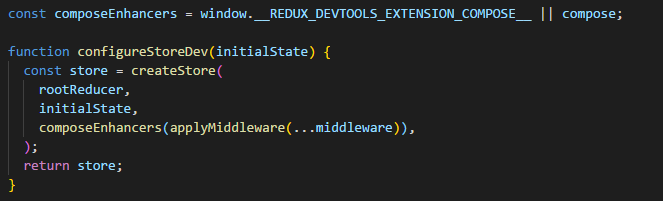
\includegraphics[width=14cm]{img/redux-devtools}\\[0.5cm]
	\end{center}
\end{figure}

Enkel het hoofdproject wordt geconnecteerd met de redux-devtools extension. Als dus gekeken wordt naar de state tree, dan is dit deze van het hoofdproject. Wanneer er meerdere projecten met elkaar gecombineerd worden, zal er nog steeds enkel de state tree van de hoofdapplicatie staan. Het zou dan ook een absolute meerwaarde zijn om deze debug tool te kunnen gebruiken met de gecombineerde state tree van beide projecten.
\autocite{devtools}

Er werd ook onderzocht of er meerdere stores mogelijk zijn voor gebruik, dan zou er per geïntegreerd project een nieuwe store bijkomen in het hoofdproject.
Het originele Flux patroon beschrijft meerdere stores in één applicatie, elke store houdt een verschillend segment van domein data vast. Dit kan problemen veroorzaken zoals een store die geforceerd wordt om te wachten op een andere store die nog geüpdatet moet worden. Dit is niet noodzakelijk zo in Redux, omdat de splitsing tussen data domeinen al bekomen wordt door het splitsen van één enkele reducer in een reeks kleinere reducers.

Het is mogelijk om meerdere verschillende Redux stores in een applicatie te hebben, maar het voorgenomen patroon bevat slechts één store. Met één store wordt het mogelijk om Redux devtools te gebruiken, het maakt persisteren van data simpeler alsook de subscription logica. Er zijn echter een aantal geldige redenen om meerdere stores te gebruiken in Redux:
\begin{itemize}
	\item Het oplossen van een performantieprobleem dat veroorzaakt wordt door het te veel updaten van een deel van de state.
	\item Het isoleren van een Redux applicatie als een component in een grotere applicatie, in dit geval is het aan te raden een store te creëren per root instantie.
\end{itemize}
Nieuwe stores aanmaken is niet het eerste waar naar gekeken moet worden, het is beter om reducer compositie toe te passen en enkel meerdere stores te gebruiken als het probleem niet opgelost kan worden op deze manier.

Gelijkaardig is het mogelijk om de store instantie aan te spreken door deze rechtstreeks te importeren, dit is eveneens geen aan te raden patroon in Redux. Wanneer een instantie van de store wordt gemaakt en geëxporteerd uit de module, dan wordt deze een singleton. Dit wil zeggen dat het moeilijker wordt om een Redux applicatie als een component van een grotere applicatie te isoleren. Er kan dan ook geen server rendering geactiveerd worden, want op de server worden er verschillende store instanties gecreëerd voor elke request die gemaakt wordt.

Het is best practice om de root component te wrappen in een <Provider> en dan gaat React Redux zorgen dat de store doorgegeven wordt naar beneden. Op deze manier moeten components geen store module importeren en worden de isolatie van een Redux app of het activeren van server rendering veel makkelijker om te implementeren.
\autocite{Redux02}

Dit staat ook beschreven in een provider patroon volgens \textcite{provider}. Veel React libraries moeten hun data doorgeven doorheen de component tree. Bijvoorbeeld, Redux moet zijn store doorgeven en React Router moet de huidige locatie doorgeven. Dit zou kunnen opgelost worden door een gedeelde, muteerbare state. Dit werkt enkel als er één state is. Wanneer er geprerenderd wordt op de server is het onmogelijk om te vertrouwen op deze implementatie. Gelukkig zorgt React voor een manier om de data van boven naar beneden te krijgen: \textit{context}. Dit kan aanzien worden als het globale object van de component tree.

Helemaal bovenaan in de app moet er dus een provider zijn. De enige rol die deze provider zal hebben is het toevoegen van gewenste data aan de context van de tree zodat alle afstammelingen ook toegang hebben tot deze data.


\paragraph{Connectie met React}
React bindings zitten echter niet standaard in Redux, eerst moet de npm-package react-redux worden geïnstalleerd. Om React en Redux samen te laten functioneren wordt gebruik gemaakt van een opsplitsing in presentationele en container components. (zie figuur 1.4 uit de lijst van figuren) 

\begin{figure}
	\begin{center}
		\caption{Verschillen tussen presentationele en container components. Verkregen van \textcite{prescon}}
		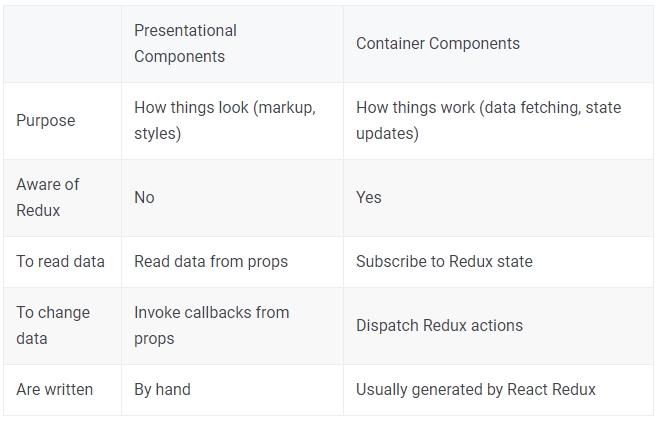
\includegraphics[width=13cm]{img/presentational-vs-container}\\[0.5cm]
	\end{center}
\end{figure}

Presentationele components zijn -zoals de naam aangeeft- prioritair voor de visualisatie. Ze verkrijgen enkel data via de props en sturen geen actions aan. 

Daar waar presentationele components gericht zijn op de visualisatie, zijn de container components gericht op het functionele aspect. Ze voorzien andere container (of presentationele) components van data en gedrag. Deze components gaan ook actions aanroepen om aan te duiden dat de data moet veranderen.  
\autocite{prescon}
\autocite{prescon2}

\subparagraph{Containers}
Het idee achter containers is dat ze de data gaan ophalen en dan de corresponderende sub-component gaan renderen. Deze data wordt gehaald uit de state en omgezet naar props voor die container. Daarna krijgen de sub-componenten de juiste props mee om hun data te renderen. 
\autocite{containercomp}

\section{Middleware}
In het Redux framework is middleware de code die zich bevindt tussen het krijgen van een request en het verzenden van een response. Express bijvoorbeeld kan CORS headers (mechanisme dat extra HTTP headers gebruikt om te laten weten aan de browser dat een web applicatie met een bepaalde oorsprong gemachtigd is om resources te gebruiken van een server met een verschillende oorsprong), logging, compressie,… toevoegen. De beste voorziening van middleware is dat het chainable is, er kan gebruik gemaakt worden van meerdere onafhankelijke third-party middleware in een enkel project.
 
Redux middleware gaat andere problemen oplossen dan de Express middleware, maar het is conceptueel dezelfde manier. Redux middleware gaat een third-party extension point voorzien tussen het dispatchen van een action en het moment dat deze action een reducer bereikt. Redux middleware wordt voornamelijk gebruikt om te loggen, voor crash reports, routing,…

Één van de voordelen van Redux is dat de veranderingen van de state voorspelbaar en transparant zijn. Elke keer een action gedispatched wordt, zal de nieuwe state berekend en opgeslagen worden. De state kan niet veranderd worden door zichzelf, maar enkel ten gevolge van een specifieke action. Via middleware is het mogelijk om elke action die verzonden wordt in de app te loggen samen met de state die erna verkregen wordt. Wanneer iets mis gaat kan er dan makkelijk teruggekeken worden in de log en kan er snel gezien worden welke action de state corrupt heeft gemaakt. De meest naïeve oplossing is om zelf de action en de volgende state te loggen elke keer de dispatch functie van de store wordt opgeroepen. Een betere oplossing is om de dispatch functie te vervangen. Met behulp van middleware kan zelf een logger geschreven worden die dan later enkel toegevoegd moet worden aan de store van de applicatie. Middleware wordt op dezelfde manier toegevoegd aan de store als de Redux devtools extension. Waar voor de Redux devtools extension een extra parameter wordt toegevoegd zal voor de middleware ook een parameter worden toegevoegd die meerdere middleware kan bevatten. 
\autocite{Redux02}

Om een betere verstandhouding van Redux te krijgen werd ook naar de voorgangers van Redux gekeken, waaronder Flux. Hieronder worden de verschillen en de gelijkenissen tussen Flux en Redux overlopen. 
Het eerste verschil is dat Flux een patroon is en Redux een library. Flux is een mooiere naam voor het observer patroon dat wat aangepast is voor React. Facebook heeft echter ook een aantal tools ontwikkeld die helpen in de implementatie van het Flux patroon. 

Flux en Redux hebben beide actions. Deze Actions kunnen vergeleken worden met events. In Flux is een action een simpel JavaScript object en dat is in het standaard geval ook zo in Redux. Wanneer er gebruik gemaakt wordt van Redux middleware kan het echter zo zijn dat actions ook functies en promises kunnen zijn. 

Met Flux is het de conventie dat er meerdere stores per applicatie zijn waarbij elke store een singleton object is. In Redux is het de conventie dat er maar één store per applicatie is. 

Flux heeft een enkele dispatcher en alle actions moeten door deze dispatcher gaan, dit is eveneens een singleton object. Een Flux applicatie kan geen meerdere dispatchers hebben. Dit is nodig omdat een Flux applicatie meerdere stores kan hebben en de afhankelijkheden tussen deze stores hebben een manager nodig, de dispatcher. In Redux is er geen dispatcher entiteit. In plaats daarvan heeft de store een dispatch proces van zichzelf. Een Redux store heeft een aantal simpele API functies, één daarvan is het dispatchen van actions.

De logica van wat er moet gebeuren wanneer er een action ontvangen wordt, zit in de store zelf bij Flux. De store heeft ook de flexibiliteit om te kiezen welke stukken data deze publiekelijk toegankelijk wil maken. Het slimste object in Flux is de store. In Redux zit de logica dan in de reducer. Een store kan niet gedefinieerd worden zonder reducer functie. Hier is het slimste object de reducer. Redux gaat ook gewoon alle data beschikbaar maken die geretourneerd wordt van de reducer. 

Nog een groot verschil is dat de state immutable is in Redux. Dit wordt makkelijk bekomen door van de reducers pure functies te maken. In Flux is hier geen restrictie, de state kan gemuteerd worden zoals gewenst.
\autocite{flux}

\section{Npm}
Om de twee projecten met elkaar te laten communiceren, wordt gebruik gemaakt van npm. De extensie op Redux zal geschreven worden en onder een eigen package gepubliceerd worden op npm, op deze manier kan de geschreven extensie aangesproken worden. 

Npm is 's werelds grootste software register met ongeveer 3 biljoen downloads per week. Het register bevat meer dan 600.000 packages. Open source developers van elk continent gebruiken npm voor het delen en lenen van packages. Veel organisaties gebruiken npm ook voor privaat development, zoals in dit onderzoek ook het geval is. 

Npm bestaat uit 3 verschillende componenten.
\begin{itemize}
	\item de website
	\item de Command Line Interface (CLI)
	\item het register
	
\end{itemize}

De website wordt gebruikt om verschillende packages te zoeken of om zelf packages op te publiceren, privaat of publiek. Deze publicatie kan via de CLI gedaan worden.

De grootste reden om npm te gebruiken is om bestaande packages aan te passen en te specialiseren naar eigen apps. Natuurlijk kan ook gebruik gemaakt worden van bestaande custom packages van andere gebruikers.
\autocite{npm}

\section{Webpack}
De meeste React-Redux projecten maken gebruik van Webpack. Webpack heeft veel populariteit gewonnen door het gebruik in React. Webpack is een statische bundelaar van modules voor JavaScript applicaties. Het kleinste project dat gebundeld kan worden met webpack bestaat uit een input en een output. Wanneer webpack bezig is met het verwerken van de applicatie, maakt het intern een \textit{dependency graph} aan. Deze wordt geconstrueerd door alle imports af te lopen. Het bundelen van modules begint bij de door gebruiker gedefinieerde entries.
\begin{description}
	\item[Een entry point] 
	 gaat aanduiden welke module webpack het eerst moet beginnen builden vanuit zijn interne dependency graph. Webpack gaat dan kijken van welke andere modules en libraries dit entry point afhankelijk is (direct en indirect). 
\end{description}

Standaard is dit entry point de index file, maar deze kan uiteraard veranderd worden of er kunnen zelfs meerdere entry points toegevoegd worden. Samen met de entry point(s) wordt meestal ook de output property gedefinieerd. Via deze property weet webpack naar waar de bundels verzonden moeten worden en hoe deze moeten heten. De standaardsetting hiervoor is de dist folder.

In de meeste applicaties zitten er echter niet enkel JavaScript files. Soms worden image imports gedaan of wordt er via een url gewerkt. Webpack verstaat echter enkel JavaScript files. Om het mogelijk te maken om andere bestandtypes te converteren in geldige modules moeten loaders toegevoegd worden. Deze modules kunnen dan gebruikt worden door de applicatie en toegevoegd worden aan de dependency graph.
\autocite{webpack} 

\begin{description}
	\item[Een loader] heeft een \textit{test} en een \textit{use} property. De test property geeft weer welke file of files die er getransformeerd moeten worden. Een use property toont aan welke loader gebruikt moet worden voor deze transformatie.
\end{description}

Loaders worden gedefinieerd in de \textit{rules} property.
Waar loaders worden gebruikt voor de transformatie van bepaalde modules, zorgen plugins ervoor dat de bundle geoptimaliseerd wordt. Plugins gaan altijd vooraf aan een require statement en kunnen later aangepast worden door extra opties toe te voegen. 

